\documentclass[twocolumn,preprintnumbers,amsmath,amssymb,notitlepage,nofootinbib,longbibliography,superscriptaddress,aps,pra,10pt]{revtex4-1}
%\documentclass[preprint,showpacs,preprintnumbers,amsmath,amssymb]{revtex4}

\usepackage{natbib}
\usepackage{graphicx}
\usepackage{dcolumn}
\usepackage{dsfont}
\usepackage{bm}
%\usepackage{float}

\usepackage[usenames, dvipsnames]{color}
\usepackage{url}
\usepackage[colorlinks=true,breaklinks=true,allcolors=blue]{hyperref}
\usepackage{microtype}
\DeclareMathOperator{\dist}{\text{dist}}

\newtheorem{theorem}{Theorem}
\newtheorem{lemma}{Lemma}

\newcommand{\ryan}[1]{\textcolor{Cyan}{RS: #1}}

\newcommand{\mk}[1]{\textcolor{Cyan}{MK: #1}}

\newcommand{\en}[1]{\textcolor{Cyan}{EN: #1}}

\newcommand{\je}[1]{\textcolor{Cyan}{JE: #1}}



\begin{document}

\title{DeepQ Decoding for Fault Tolerant Quantum Computation}

\author{Ryan Sweke}
\affiliation{\mbox{Dahlem Center for Complex Quantum Systems, Freie Universit\"{a}t Berlin, 14195 Berlin, Germany}}
\author{Markus S. Kesselring}
\affiliation{\mbox{Dahlem Center for Complex Quantum Systems, Freie Universit\"{a}t Berlin, 14195 Berlin, Germany}}
\author{Evert P.L. van Nieuwenburg}
\affiliation{\mbox{Institute for Quantum Information and Matter, Caltech, Pasadena, CA 91125, USA}}
\author{Jens Eisert}
\affiliation{\mbox{Dahlem Center for Complex Quantum Systems, Freie Universit\"{a}t Berlin, 14195 Berlin, Germany}}


\date{\today}


\begin{abstract}
	Topological error correcting codes, and particularly the surface code, currently provide the most feasible roadmap towards large-scale fault tolerant quantum computation.
	As such, obtaining fast and flexible decoding algorithms for these codes, within the experimentally relevant context of faulty syndrome measurements, is of critical importance.
	In this work we show that the problem of decoding such codes, in the full fault tolerant setting, can be naturally reformulated as a process of repeated interactions between a decoding agent and a code environment, to which the machinery of reinforcement learning can be applied to obtain decoding agents.
	As a demonstration, by using deepQ learning, we obtain fast decoding agents for the surface code, for a variety of noise-models, within the fully fault tolerant setting.
\end{abstract}

\maketitle


\section{Introduction}\label{s:introduction}

	In order to implement large scale quantum algorithms it is necessary to be able to store and manipulate quantum information in a manner that is robust with respect to the unavoidable errors introduced through the interaction of physical qubits with a noisy environment.
	A typical strategy for achieving such robustness is to encode a single logical qubit into the state of many physical qubits, via a quantum error correcting code, from which it may be possible to actively diagnose and correct errors that might occur~\cite{Terhal15,Campbell17}.
	While many quantum error correcting codes exist, topological quantum codes~\cite{Kitaev03, Dennis02, Preskill17lectures, Nayak08, Pachos12, Terhal15, Brown16, Campbell17} in which only local operations are required to diagnose and correct errors, are of particular interest as a result of their experimental feasibility~\cite{Reed12, Barends14, Nigg14, Corcoles15, Albrecht16, Takita16, Linke17}.
	Recently the surface code has emerged as an espescially promising code for large scale fault tolerant quantum computation, due to the combination of its comparitively low overhead and locality requirements, coupled with the availability of convenient strategies for the implementation of all required logical gates.

	Within any such code based strategy for fault tolerant quantum compuation, decoding algorithms play a critical role.
	At a high level, throughout the course of a computation these algorithms take as input the outcome of diagnostic syndrome measurements and should provide as output suggested corrections for any errors which might have occurred, which can then be tracked through the computation and later used to apply corrections to any obtained results.
	It is particularly important to note that in any physically realistic setting the required syndrome measurements are themselves obtained via small quantum circuits, and are therefore also generically faulty.
	As such, while the setting of perfect syndrome measurements provides a good test-bed for the development of decoding algorithms, any decoding algorithm which aims to be experimentally feasible should also be capable of dealing with such faulty syndrome measurements.
	Additionally, such algorithms should also be capable of dealing with experimentally relevant noise models, as well as be fast enought to not present a bottleneck to the execution of computations, even as the size of the code scales to larger code distances.

	Due to the importance of decoding algorithms for fault tolerant quantum computation, many different approaches have been developed, each of which tries to satisfy as many of the experimentally required criterion as possible.
	Perhaps most prominent are algorithms based on minimum-weight perfect matching subroutines~\cite{Fowler13}, however alternative approaches based on techniques such as the renormalization group~\cite{Duclos2010} and locally operating cellular automata~\cite{Herold15} have also been put forward.
	Furthermore, recently techniques from classical machine learning have begun to find application in diverse areas of quantum physics - such as in the efficient representation of many-body quantum states, the identification of phase transitions, and the autonomous design of novel experimental setups \mk{TODO: add citations} - and various neural-network based decoders have also been proposed~\cite{Torlai10, Varsamopoulos17, Krastanov17, Breuckmann18, Baireuther18a, Baireuther18b, Ni18}.
	However, despite the diversity of decoding algorithms now available, there is not as of yet an algorithm which clearly satisifes all the required criteria, or a clear consensus as to which technique would be the most experimentally feasible in any given experimental context.
	In particular, while the so-far proposed neural network decoders promise extremely fast decoding times, flexibility with respect to the underlying noise model and the potential to scale to large code distances, all such decoders are so far restricted either to the setting of perfect syndrome measurements, or to the setting in which one is trying to store a logical qubit as long as possible, without the requirement of performing a subsequent logical gate.
	As such, while this approach seems promising, there remains room for improvement and generalization.

	Simultaneously, the last few years have also seen extremely impressive advances in the development of deep reinforcement learning algorithms, which have allowed for the training of neural network based agents capable of obtaining super-human performance in domains such as Atari~\cite{Mnih15}, Chess~\cite{Silver17a} and Go~\cite{Silver17b}.
	These techniques are particularly powerful in situations where it is necessary to learn strategies for complex sequential decision making, involving consideration of the future effects of ones actions.
	At a surface level, the problem of decoding within the context of fault-tolerant quantum computation seems like exactly such a setting and as such it natural to ask to what extent reinforcement learning techniques could be used to obtain decoding agents, and what advantages such agents might have over existing approaches.
	In this work we set out to provide answers to these questions.

	In particular, we reformulate the problem of decoding within the setting of fault-tolerant quantum computation as a process of sequential competitive interaction between a decoding agent and a code environment.
	This reframing provides a conceptual framework which allows for the application of various deep reinforcement learning algorithms to obtain neural network based decoding agents.
	As a proof-of-principle, we then utilize to deepQ learning to obtain fast surface code decoders, for a variety of noise models, within the fully fault-tolerant setting.
	These results then provide a foundation for extension via both more sophisticated reinforcement learning techniques and more sophisticated neural network models.

	In this work we begin by providing an introductory overview of the surface code in Section~\ref{s:the_surface_code}, before presenting a description of the decoding problem for fault-tolerant quantum computation in Section~\ref{s:the_decoding_problem}.
	After a brief introduction to the formalism of reinforcement learning and $Q$-functions in Section~\ref{s:reinforcement_learning} we are then able to provide the conceptual reframing of decoding as a reinforcement learning problem in Section~\ref{s:decoding_as_rl}, which is one of the primary results of this work.
	In Section~\ref{s:results} we then present deepQ surface code decoders for a variety of noise models, before finally in Section~\ref{s:conclusions} discussing both the advantages and disadvantages of the approach presented here, along with various potential strategies for building upon the results presented in this work.

\section{The Surface Code}\label{s:the_surface_code}

	    We begin by providing a brief description of the surface code. 
        The framework and methods presented in this work are not restricted to the surface code, and could be applied to any stabilizer code, but we choose to restrict ourselves to this code here for both simplicity of presentation and experimental relevance. 
        We will focus on presenting the elements of the surface code necessary for understanding the decoding problem, in the process omitting many details, for a more detailed treatment refer to refs \textit{a,b, and c}.

        As illustrated in Fig. \ref{f:surface_code}, we will consider $d\times d$ lattices with a \textit{physical data qubit} on each vertex $v$, such that the collective state of all qubits on the lattice is an element of the Hilbert space $\mathcal{H} = \mathbb{C}^{2^{(d\times d)}}$. 
        We associate stabilizer operators with each coloured plaquette of the lattice.
        Stabilizers on blue (orange) plaquettes are operators which apply Pauli X (Z) flips to all qubits on the vertices of the plaquette. 
        Specifically, denoting the set of all blue (orange) plaquettes as $B_p$ ($O_p$) we define the stabilizer $S_p$ on plaquette $p$ as,

        \begin{equation}\label{e:stabilizer_definition}
            S_p = \bigotimes_{v\in p} \sigma_v \quad \text{where   }   \begin{cases}
                                                                        \sigma_v = X_v \quad \text{if } p \in B_p,\\
                                                                         \sigma_v = Z_v \quad \text{if } p \in O_p.
                                                                     \end{cases}
        \end{equation}
        All stabilizers are mutually commuting and have eigenvalues $\pm 1$.
        If we define the Hamiltonian $H = -\sum_p S_p$, then the surface code $\mathcal{H}_\mathrm{sc} \subset \mathcal{H}$ is the ground state space of this Hamiltonian, which is the space consisting only of simultaneous $+1$ eigenstates of all the stabilizer operators. 
        This subspace is two dimensional, i.e. $\mathcal{H}_\mathrm{sc} \simeq \mathbb{C}^2$, and as a result we can encode a single \textit{logical qubit} into this code space.
        Logical operators are then operators which preserve the code space and manipulate the state of the logical qubit. As shown in Fig. \ref{f:surface_code}, logical $X$ ($Z$) operators, denoted $X_L$ ($Z_L$), are continuous strings of single vertex $X$ ($Z$) operators which connect the top and bottom (left and right) boundary of the lattice.


        \begin{figure}
            \centering
            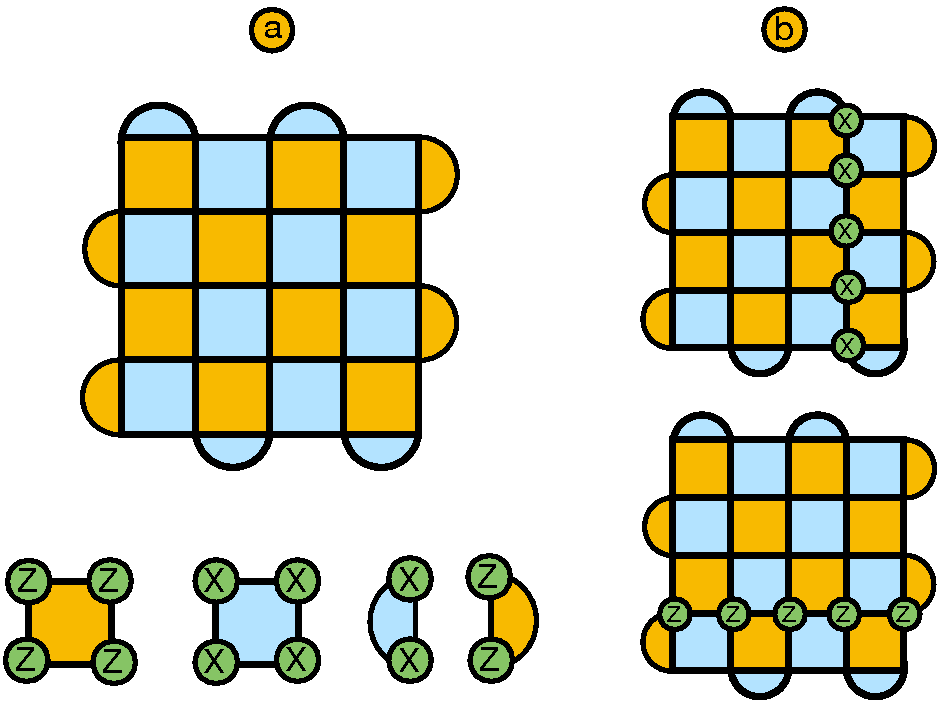
\includegraphics[width=0.8\linewidth]{figures/surface_code.pdf}
            \caption{An overview of the $5 \times 5$ surface code. (a) We consider square lattices, with a data qubit on each vertex of the lattice. The coloured plaquettes indicate stabilizer operators as defined in Eq. \eqref{e:stabilizer_definition}. (b) Logical $X_L$ and $Z_L$ operators for the surface code are given by continuous strings of single qubit $X$ or $Z$ operators connecting the top and bottom or left and right boundaries of the code respectively.}\label{f:surface_code}
        \end{figure}

        To illustrate the motivation behind such an encoding, let's examine the consequences of a single qubit Pauli flip on a physical data qubit. 
        If we assume that the initial state $|\psi\rangle \in \mathcal{H}_\mathrm{sc}$ is an element of the code space, then the subsequent state $|\psi'\rangle$ will no longer be an element of the code space.
        In particular $|\psi'\rangle$ will be an eigenstate with eigenvalue $-1$ of at least one stabilizer. 
        We say that $|\psi'\rangle$ violates these stabilizers, as illustrated by red circles in Fig.~\ref{f:surface_code_examples}~(a).
        The \textit{syndrome} of a state is the string encoding the outcomes of a simultaneous measurement of all the stabilizers, each of which takes the value $\pm 1$.
        As such, unlike a truly single qubit encoding of a quantum state, if a Pauli flip error occurs on a single physical data qubit, we may be able to identify and correct this error, in the process conserving the logical qubit state, by examining the syndrome of the post-error state. 
        This process of \textit{decoding} is discussed in the next section.

        \begin{figure}
            \centering
            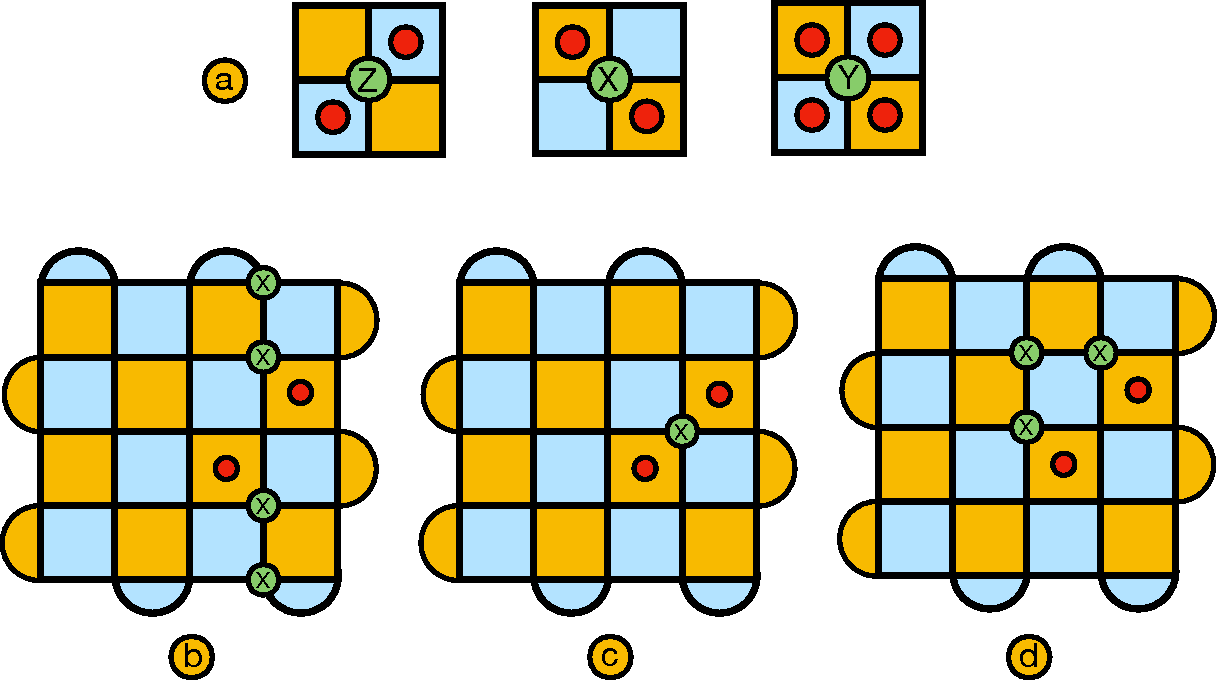
\includegraphics[width=1\linewidth]{figures/surface_code_examples.pdf}
            \caption{(a) Single qubit Pauli flips violate surrounding stabilizers. (b-d) Strings of Pauli flips only violate stabilizers at the endpoint of the string. Multiple error configurations can give rise to the same syndrome. They can differ by stabilizers, as for example in (c) and (d), or by logical operators, see (b) and (c).}\label{f:surface_code_examples}
        \end{figure}


\section{The Decoding Problem}\label{s:the_decoding_problem}

    Given the foundations from the previous section, we are able to succinctly state a simple preliminary version of the decoding problem:\newline

    \noindent\textit{Assume that at} $t=0$  \textit{one is given a state} $|\psi\rangle = \alpha |0_L\rangle + \beta |1_L\rangle \in \mathcal{H}_{\mathrm{sc}}.$ \textit{At some time }$t_1>0$ \textit{a syndrome measurement is performed which indicates that one or more stabilizers are violated - i.e. some errors have occurred on physical data qubits. From the given syndrome, determine a set of corrections which should be applied to the code lattice such that the subsequent state} $|\psi'\rangle$ \textit{is equal to the initial state} $|\psi\rangle.$ \newline

    \begin{figure*}
      \centering
      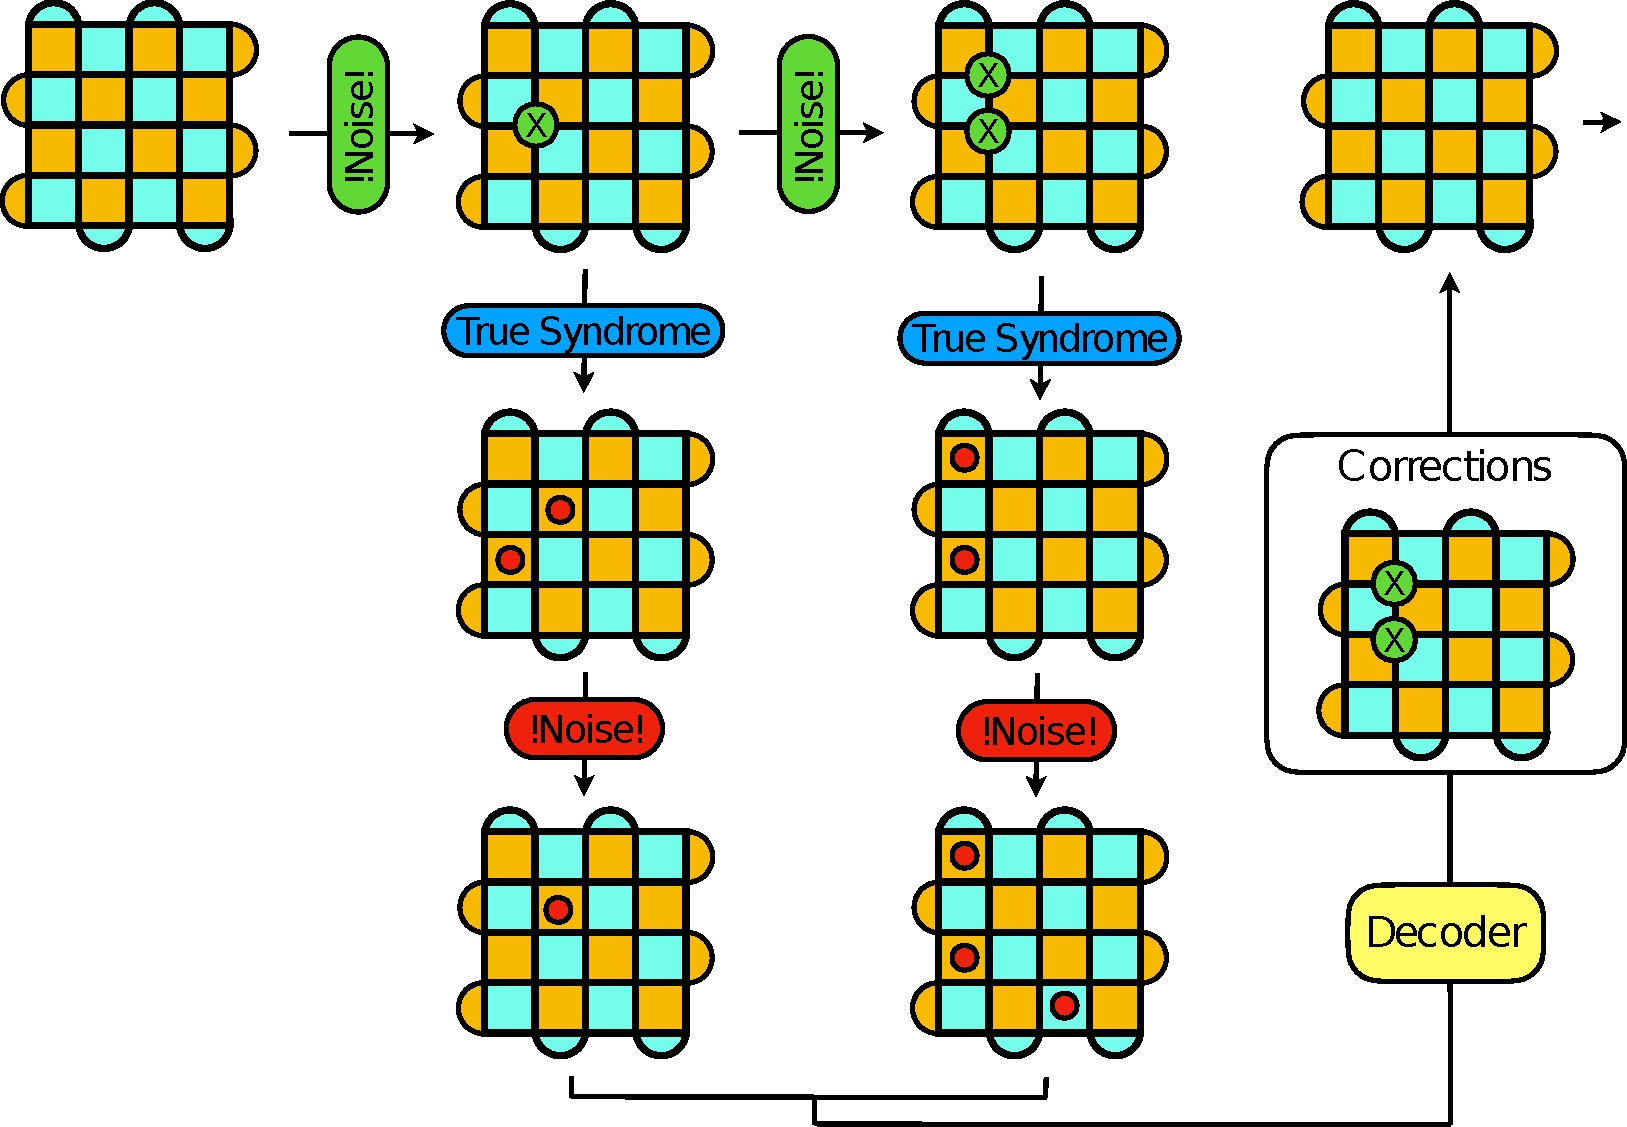
\includegraphics[width=0.65\textwidth]{figures/decoding_problem.pdf}
      \caption{A typical decoding cycle is illustrated for the simplified faulty measurements scenario in which one imagines each time step consisting of an initial physical error process generating errors on the data qubits, followed by a second measurement error process which corrupts the true syndrome. The decoding algorithm then has access to a sequence of potentially faulty syndromes.}\label{f:decoding_problem}
    \end{figure*}

    \noindent Before proceeding to discuss more subtle and technical versions of the decoding problem, let's examine why even the above problem is indeed potentially difficult.
    The most important observation is that the map from error configurations to syndromes is many-to-one, i.e. many different sets of errors can lead to the same syndrome.
    As an example, consider the error configurations illustrated in lattices (b), (c) and (d) of Fig.~\ref{f:surface_code_examples}, all of which lead to the same syndrome.
    If the probability of an error on a single physical data qubit is low, given such a syndrome one might reasonably assume that the error in lattice (c) occurred, as one error on a single qubit is a more likely event than errors on multiple qubits.
    Given this reasoning, one might then suggest to correct by applying an $X$ flip on the physical data qubit in the third row and fourth column.
    If indeed the error in lattice (c) occurred then this would be the correct operation.
    However, if the error in lattice (d) occurred, then the combination of the original error with the correction would implement a stabilizer.
    As the original state was a simultaneous $+1$ eigenstate of all the stabilizers, stabilizer operators act trivially on logical states, and hence the proposed correction preserves the initial logical state.
    Finally, if the error in lattice (b) occurred, then the combination of the original error with the correction would implement the logical $X_L$ gate.
    As a result, even though the post-correction state is back in the code space, it will be in a different state to the original state and the information we were trying to preserve would have been corrupted.
    From this simple example one can see that most often solving the decoding problem as stated above involves deciding, given an inherently ambiguous syndrome and (possibly imperfect) knowledge of the underlying error model, which error configuration was most likely to have occurred.

    In addition to the inherent difficulty resulting from syndrome ambiguity, in experimental settings the process of extracting the syndrome is also subject to noise, and as such the syndrome one receives may also contain errors.
    In practice, each stabilizer is associated with a physical ancilla qubit, and the syndrome value for that particular stabilizer is obtained by first executing a small quantum circuit which entangles the ancilla with each of the physical data qubits on which the corresponding stabilizer is supported, before extracting the syndrome value via a measurement of the ancilla qubit.
    In order to fully account for errors during the process of syndrome extraction one should therefore model this entire circuit, in which errors can occur on both the data qubits and ancilla qubits at each time step, and importantly, errors on the ancilla qubits can propagate onto the data qubits via the required entangling gates.
    However, the essential aspect of the additional difficulty from faulty syndrome measurements can be phenomenologically modelled by imagining each time step as consisting of two distinct error processes, as illustrated in Fig.~\ref{f:decoding_problem}.
    In the first error process, an error occurs on each data qubit with some probability.
    One then imagines extracting the perfect syndrome before a second error process occurs, in which with a given probability an error occurs on each stabilizer measurement outcome.
    As single syndromes are no longer reliable, decoding within the setting of faulty syndromes typically requires providing the decoding algorithm with multiple sequential syndromes.

    Finally, in the context of surface code based fault tolerant quantum computing, all logical gates are implemented either via protocols which also involve an inherent decoding procedure or do not spread errors. 
    To be specific, it is sufficient to be able to implement both Clifford and $T$ gates.
    In contemporary proposals for surface code based quantum computing protocols are known for implementing Clifford gates transversally, via code deformation or via lattice surgery.
    While transversal gates do not spread errors, code deformation and lattice surgery require decoding cycles.
    Non-Clifford gates, such as the $T$ gate, can be performed fault tolerantly via gate teleportation using magic states. 
    High quality magic states can be obtained via magic state distillation, which requires only Clifford gates and initially faulty magic states.
    As such the goal of decoding idling logical qubits within a quantum computation should be to suppress errors to the extent that any of the above procedures can succeed with high probability.
    Therefore, we can relax the requirement that the decoding process should return the post-error state to the initial state in the code space.
    In Section \ref{s:decoding_as_rl} we discuss a proxy criterion for decoding success within this framework.


\section{Reinforcement Learning and q-Functions}\label{s:reinforcement_learning}

    In this section we shift focus and introduce some of the fundamental concepts of reinforcement learning and $q$-functions, which will be crucial to our conceptual reframing of the decoding problem in Section \ref{s:decoding_as_rl}. 
    Again, we will omit many interesting details, which can be found in the standard textbook. 
    As illustrated in Fig. \ref{f:agent_environment}, we imagine an agent interacting with some environment in discrete time steps. 
    In each time step $t$ the agent is in some state $S_t$, which is generically a combination of its knowledge of the environment $S_{E,t}$, its memory of its own previous actions, and possibly the state of additional internal variables. 
    From this state the agent must then choose some valid action $A_t$, which it applies to the environment. 
    In response to this action, via some process which is typically not directly known by the agent, the environment updates and provides the agent with a potentially reduced description of its new state $S_{E,t+1}$ (i.e. a description of the part of the environment which is \textit{visible} to the agent), along with a a scalar reward $R_{t+1}$ and a boolean signal which indicates whether the game is over - i.e. whether the agent has failed, died or lost. 
    In principal it is also possible to imagine settings in which the sequence of interactions can carry on indefinitely, but we will consider here only episodic actions, which end once the environment is placed into a terminal state (which may not be unique) by the actions of the agent. 
    Generically, we consider to goal of the agent to be to avoid dying, while accumulating as much reward as possible.

    Typically the way that the agent chooses its action, the way that the environment is effected by the action, and the reward that is generated can all be stochastic, and in the context of finite state and action spaces, denoted $\mathcal{S}$ and $\mathcal{A}$ respectively, this process can be formalized within the framework of finite Markov decision processes (FMDP):

    \begin{equation}
        p(s',r|s,a) \equiv \mathrm{pr}(S_t = s',R_t = r|S_{t-1} = s, A_{t-1} = a).
    \end{equation}
    To formalize the decision making process of the agent, we define an agent's \textit{policy} $\pi$, in essence the agent's strategy, as a mapping from states to probabilities of specific actions - i.e. $\pi(a|s)$ is the probability that $A_t = a$ if $S_t = s$. 
    For FMDP's we then define the \textit{value} of a state $s$ under policy $\pi$ as,

    \begin{equation}
        v_{\pi}(s) = \mathbb{E}_{\pi}[G_t|S_t = s]  = \mathbb{E}_{\pi} \Big[\sum_{k = 0}^{\infty}\gamma^k R_{t+k+1}\Big| S_t = s \Big] 
    \end{equation}
    $\forall S_t \in \mathcal{S}$, where $G_t$ is the discounted return (discounted cumulative reward), with discount factor $0 \leq \gamma \leq 1$, and in practice the infinite sum terminates whenever state $S_{t+k+1}$ is a terminal state. 
    We call $v$ the \textit{state-value function}, which provides the expected discounted cumulative reward the agent would obtain when following policy $\pi$ from state $s$. 
    It is an important conceptual point to note that by using the metric of the discounted cumulative reward the value of any given state depends not only on the immediate rewards an agent would obtain from following a specific policy, and hence strategies which involve some element of successful future planning may lead to higher state values. 
    As such, we see that the value of a state with respect to a given policy reflects accurately the ability of an agent to achieve its long-term goals when following that policy from that state. 
    Similarly, we can define the \textit{action-value function}  (referred to as the $q$-function) for policy $\pi$ via:

    \begin{align}
        q_{\pi}(s,a) &= \mathbb{E}_{\pi}[G_t|S_t = s, A_t = a]  \\
        & = \mathbb{E}_{\pi} \Big[\sum_{k = 0}^{\infty}\gamma^k R_{t+k+1}\Big| S_t = s, A_t = a \Big]
    \end{align}
    Clearly, the $q$ function with respect to a given policy is conceptually similar to the value function, except that it provides the value (expected discounted cumulative reward) associated with following a given policy after taking a certain action from a certain state. 
    Importantly, value functions allow us to place an order over policies, i.e. $\pi > \pi' \iff v_{\pi}(s) > v_{\pi'}(s)\quad \forall s \in \mathcal{S} $. 
    Given such an ordering we can then define an optimal policy $\pi^*$, with respect to which the action-value function will be the unique solution of the following system of equations:

    \begin{figure}
      \centering
          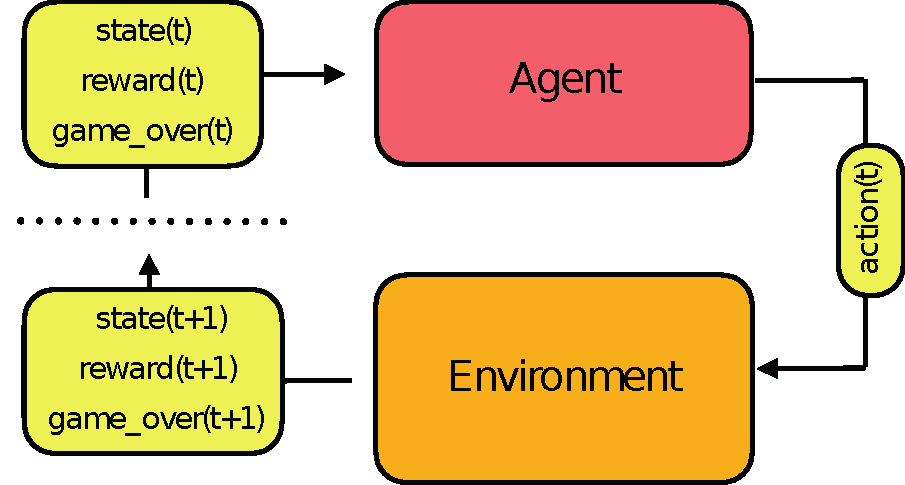
\includegraphics[width=0.4\textwidth]{figures/agent_environment.pdf}
      \caption{An illustration of the signals passed between an agent and the environment through the duration of a sequential turn based episode.}\label{f:agent_environment}
    \end{figure}

    \begin{equation}\label{e:fixed_point}
        q_*(s,a) = \mathbb{E}\big[R_{t+1} + \gamma\max_{a'}q_{*}(S_{t+1},a')\big|S_t = s, A_t = a \big].
    \end{equation}
    Note that given the optimal $q$-function it is easy to obtain the optimal strategy; When in a given state $s$ simply choose the action $a = \mathrm{argmax}_{a'}[q_*(s,a')]$.

    It is now possible to introduce the idea of iterative $q$-learning as a tool for obtaining optimal $q$-functions via experience gained from interaction with a given environment. 
    Starting from an arbitrary initial $q$-function, the idea is to use Eqn. \eqref{e:fixed_point} as the basis for an update method, via which the $q$-function is updated while an agent uses this $q$-function (possibly in conjunction with additional exploratory strategies) to interact with the environment. 
    The goal is that this $q$ function will eventually converge to $q_*$, which is a stationary point of Eqn. \eqref{e:fixed_point}. 
    Under certain conditions, it can in fact be proven that this will be the case.

    More specifically, for \textit{deepQ} learning we parametrize $q$ with a neural network, and use Eqn. \eqref{e:fixed_point} to construct the cost function from which the network weights can be updated via some gradient descent method. In particular, we let the agent interact with the environment via an $\epsilon$-greedy exploration policy, in the process generating experience-tuples of the following form:

    \begin{equation}
        [S_t,A_t,R_{t+1},S_{t+1}]
    \end{equation}
    From these tuples we can construct a loss on which to train the $q$-network, by using the cost function:

    \begin{align} 
    C &= y_{\mathrm{pred}} - y_{\mathrm{true}}\\
    &= q(S_t,A_t) - \big[R_{t+1} + \gamma\max_{a'}q(S_{t+1},a') \big]
    \end{align}
    which, by comparison with \eqref{e:fixed_point}, will be 0 only for the optimal policy. Unfortunately, despite the simplicity of the idea, in practice a variety of tricks - such as batched experience replay, separate active and target $q$-networks, double-$q$ learning and dueling networks - are required to achieve stable $q$-learning. We refer to the relevant references, or to the associated code repository, for details.



\section{Decoding as a Reinforcement Learning Problem}\label{s:decoding_as_rl}
\section{Results}\label{s:results}
\section{Conclusion}\label{s:conclusions}


\begin{acknowledgments}
	The authors gratefully acknowledge helpful and insightful discussions with Daniel Litinski, Nicolas Delfosse, Paul Baireuther, and Hendrik Poulsen Nautrup.
	Additionally, the authors would like to thank J\"{o}rg Behrmann for incredible technical support, without which this work would not have been possible.
	RS\ acknowledges the financial support of the Alexander von Humboldt foundation.
	MSK\ is supported by the DFG (CRC183, project B02).
	EvN\ is supported by ...
	JE\ is supported by DFG (CRC 183, EI 519/14-1, and EI 519/7-1), the ERC (TAQ), the Templeton Foundation, and the BMBF (Q.com).
\end{acknowledgments}

\bibliography{dq}

\end{document}
